\documentclass[border=4pt]{standalone}
\usepackage{mathptmx}
\usepackage{tikz}
\usetikzlibrary{positioning,arrows.meta,calc,fit}
\definecolor{frozenfill}{HTML}{F2F2F2}\definecolor{frozenline}{HTML}{8C8C8C}
\definecolor{trainfill}{HTML}{F7E3D3}\definecolor{trainline}{HTML}{B5652B}
\definecolor{salfill}{HTML}{E1E9F3}\definecolor{salline}{HTML}{4C72B0}
\tikzset{
  blk/.style={draw, rounded corners=1.5pt, line width=0.5pt, minimum height=11mm, align=center, font=\small, text width=30mm},
  frozen/.style={blk, fill=frozenfill, draw=frozenline},
  trained/.style={blk, fill=trainfill, draw=trainline},
  sal/.style={blk, fill=salfill, draw=salline},
  arr/.style={-{Stealth[length=2.2mm]}, line width=0.5pt},
  note/.style={font=\footnotesize\itshape, text=black!65}
}
\begin{document}\hyphenpenalty=10000\exhyphenpenalty=10000
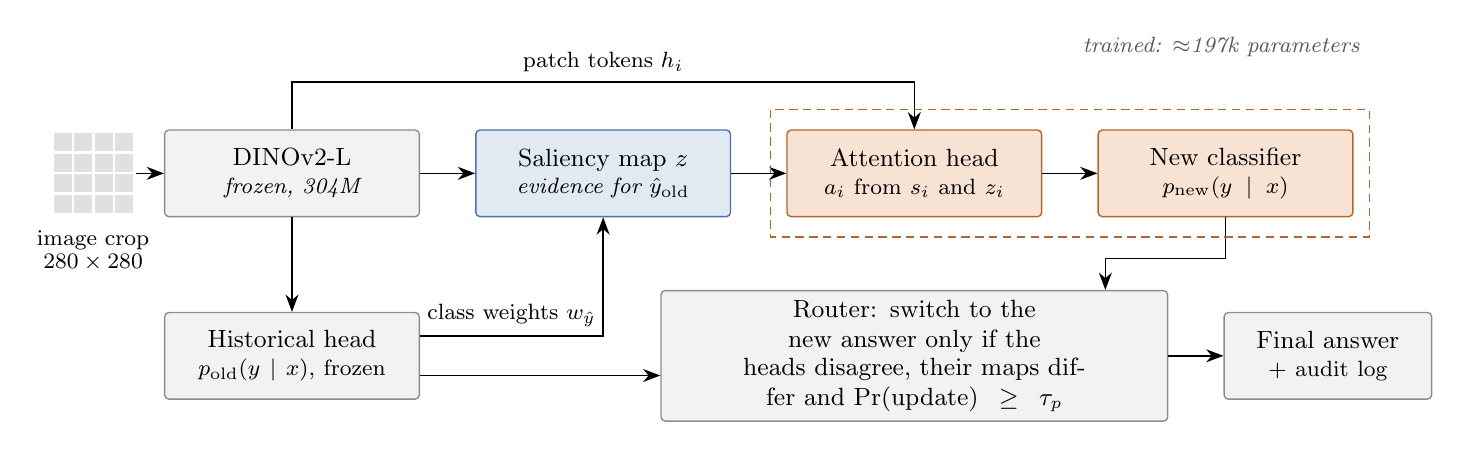
\begin{tikzpicture}[node distance=8mm and 7mm]
% image as a 4x4 grid
\begin{scope}[shift={(0,0)}]
  \foreach \i in {0,...,3} \foreach \j in {0,...,3} {\fill[black!12] (\i*2.6mm,\j*2.6mm) rectangle ++(2.3mm,2.3mm);}
  \coordinate (imgc) at (5mm,5mm);
\end{scope}
\node[font=\footnotesize, align=center, below=1mm] at (5mm,0) {image crop\\[-1pt]$280\times280$};
\node[frozen, right=9mm of imgc] (bb) {DINOv2-L\\[-1pt]{\footnotesize\itshape frozen, 304M}};
\node[sal, right=of bb] (z) {Saliency map $z$\\[-1pt]{\footnotesize\itshape evidence for $\hat{y}_{\mathrm{old}}$}};
\node[trained, right=of z] (head) {Attention head\\[-1pt]{\footnotesize $a_i$ from $s_i$ and $z_i$}};
\node[trained, right=of head] (new) {New classifier\\[-1pt]{\footnotesize $p_{\mathrm{new}}(y\mid x)$}};
\node[frozen, below=12mm of bb] (old) {Historical head\\[-1pt]{\footnotesize $p_{\mathrm{old}}(y\mid x)$, frozen}};
\node[frozen, text width=62mm] (router) at (old -| head) {Router: switch to the new answer only if the\\[-1pt]heads disagree, their maps differ and $\Pr(\mathrm{update})\geq\tau_p$};
\node[frozen, right=of router, text width=24mm] (out) {Final answer\\[-1pt]{\footnotesize + audit log}};
\draw[arr] ($(imgc)+(5.5mm,0)$) -- (bb);
\draw[arr] (bb) -- (z); \draw[arr] (z) -- (head); \draw[arr] (head) -- (new);
\draw[arr] (bb) -- (old);
\draw[arr] ($(old.east)+(0,-2.5mm)$) -- ($(router.west)+(0,-2.5mm)$);
\draw[arr] ($(old.east)+(0,2.5mm)$) -| node[pos=0.25, above, font=\footnotesize] {class weights $w_{\hat{y}}$} (z.south);
\draw[arr] (bb.north) -- ++(0,6mm) -| node[pos=0.25, above, font=\footnotesize] {patch tokens $h_i$} (head.north);
\draw[arr] (new.south) |- ($(router.north east)+(0,4mm)$) -- ($(router.north east)+(-8mm,4mm)$) -- ($(router.north east)+(-8mm,0)$);
\draw[arr] (router) -- (out);
\draw[densely dashed, line width=0.4pt, trainline] ($(head.north west)+(-2mm,2.5mm)$) rectangle ($(new.south east)+(2mm,-2.5mm)$);
\node[note, anchor=south east] at ($(new.north east)+(2mm,8mm)$) {trained: $\approx$197k parameters};
\end{tikzpicture}
\end{document}
